% !TeX root = ../thesis.tex
\chapter{Long-Time stability of small FPUT solitary waves}
\label{chp:long-time-stability}
\pagestyle{myheadings}

\section{Introduction}

As shown in earlier work, there exists a wave solution of the FPUT lattice whose profile is well approximated by that of the kink solution to the (defocusing) mKdV. We are now interested in studying the stability of this wave solution on the FPUT lattice. The equations of motion on the lattice are given by 
\begin{equation}\label{fput-lattice-equations}
	\ddot x_n = V'(x_{n+1} - x_n) - V'(x_n - x_{n-1}), \quad n \in \Z.
\end{equation}
where \(V\) is the interaction potential between neighboring particles and \(\dot{\hspace{0.5em}}\) denotes the derivative with respect to the time \(t\in \mathbb{R}\). \Cref{fput-lattice-equations} can be rewritten in the strain variables \(u_n := x_{n+1} - x_n\) as follows
\begin{equation}\label{fput-lattice-equations-strain-variables}
	\ddot{u}_n = V'(u_{n+1}) - 2 V'(u_n) + V'(u_{n-1}), \quad n \in \Z
\end{equation}
The moving wave solution in \cref{fput-lattice-equations} corresponds to a kink solution in \cref{fput-lattice-equations-strain-variables}.

For the case where \(V\) is of the form \(V(u) = \frac 1 2 u^2 + \frac{\epsilon^2}{p+1} u^{p+1}\) for \(p\geq 2\), the generalized KdV equation given by 
\begin{equation}\label{generalized-KdV}
	2 \partial_TW + \frac 1 {12} \partial_X^3 W + \partial_X(W^p) = 0,\quad X\in\R
\end{equation} 
serves as a modulation equation for solutions of \cref{fput-lattice-equations-strain-variables} \cite{bambusi2006metastability,friesecke1999solitary}. That is, for a local solution \(W\in C([-\tau_0,\tau_0],H^s(\R))\) of \cref{generalized-KdV} there exist positive constants \(\epsilon_0\) and \(C_0\) such that, for all \(\epsilon \in (0,\epsilon_0)\), when initial data \((u_{\mathrm{in} }, \dot u_{\mathrm{in}})\in\ell^2(\R)\) satisfy
\begin{equation}
	\|u_{\mathrm{in}} - W(\epsilon\cdot, 0) \|_{\ell^2} + \| \dot u_{\mathrm{in}} + \epsilon \partial_X W(\epsilon\cdot, 0) \|_{\ell^2} \leq \epsilon^{3/2},
\end{equation}
the unique solution to \cref{fput-lattice-equations-strain-variables} with initial data \((u_{\mathrm{in} }, \dot u_{\mathrm{in}})\) belongs to \(C^1([-\tau_0\epsilon^{-3}, \tau_0 \epsilon^{-3}];\allowbreak \ell^2(\Z))\) and satisfies 
\begin{multline}
	\|u(t) - W(\epsilon (\cdot - t),\epsilon^3 t)\|_{\ell^2(\Z)} + \| \dot u(t) + \epsilon \partial_X W(\epsilon(\cdot - t), \epsilon^3 t) \|_{\ell^2(\Z)} \leq C_0 \epsilon^{3/2}, \\ t\in[-\tau_0 \epsilon^{-3},\tau_0 \epsilon^{-3}].
\end{multline}
Furthermore, the approximation can also be extended to include counter-propagating solutions of the KdV in the case where \(p=2\) \cite{schneider2000counter}.

The KdV approximation was extended to longer time scales on the order of \(\epsilon^{-3}|\log(\epsilon)|\) by Khan and Pelinovsky in order to deduce the nonlinear metastability of small FPUT solitary waves from the orbital stability of the corresponding KdV solitary waves \cite{khan2017long}.

We consider the FPUT with potential
\begin{equation}\label{truncated-potential}
	V(u) = \frac 1 2 u^2 - \frac{1} {24} u^4.
\end{equation}
We will introduce an ansatz that solutions of the FPUT with this potential can be well-approximated by counter-propagating solutions of mKdV equations.

The technique of the proof follows roughly from \cite{schneider2000counter,khan2017long} and is roughly sketched out as follows. First the system is rewritten into a Hamiltonian system on a Hilbert space, \(H\):
\begin{equation}\label{hamiltonian-system}
	\dot X(t) = J \mcH'(X)
\end{equation}
where \(J:H\to H\) is a skew symmetric operator and \(\mcH\) is the Hamiltonian, where we take \(\mcH'(X) = LX + N(X)\) with \(L:= \mcH'(0)\). We introduce some ansatz \(\tilde X_\epsilon\) which is an approximate solution to \cref{hamiltonian-system} in the sense that 
\begin{equation}
	\mathrm{Res}(t) := J[L\tilde X_\epsilon(t)  + N(\tilde X_\epsilon(t))] - \dot{\tilde {X_\epsilon}}(t) 
\end{equation}
has norm of order \(\epsilon^\alpha\) for \(\alpha > 0\)  for all time \(t\). The approximate solution will be ``small-amplitude" in the sense that \(\| \tilde X_\epsilon \| = \mathcal O(\epsilon^k)\) for \(k > 0 \). Then we can write the evolution equation for the \(R(t) = X(t) - \tilde X_\epsilon(t)\) as 
\begin{equation}\label{hamiltonian-system-2}
	\dot R(t) = J[L + N'(\tilde X_\epsilon(t))]R(t) + \mathrm{Res}(t) + \mathcal N(\tilde X_\epsilon, R)
\end{equation}
with \(\mathcal N( X_\epsilon, R) := J[N(\tilde X_\epsilon +R) - N(\tilde X_\epsilon) - N'(\tilde X_\epsilon)R]\). The goal is then to show that \(R(t)\) remains small for long periods of time so that the approximation \(X \approx \tilde X_\epsilon\) is valid for that time. The standard way to prove this is to find a suitable energy function to control the norm of \(R\) with. If \(L + N'(\tilde X_\epsilon(t))\) is self-adjoint, then \cref{hamiltonian-system-2} is up to first order a linear, non-autonomous, Hamiltonian system with Hamiltonian \(\mcH_1(R, t) = \frac 1 2 \langle (L+N'(\tilde X_\epsilon)) R, R\rangle\). Therefore, \(\mcE(t) := \mcH_1(R(t),t)\) serves as a natural choice of energy function for \cref{hamiltonian-system-2}. Hence, if one shows that \( \| R\|^2\lesssim\mcE(t)\) and that  \(\|\mathcal N(\tilde X_\epsilon, R) \| \lesssim \epsilon^{k+2} \mcE(t)\), then can show that \(\mcS(t) = \mcE(t)^{1/2}\) satisfies
\begin{equation}
	|\dot \mcS (t) | \lesssim \epsilon^{\alpha} + \epsilon^{k+2}\mcS(t).
\end{equation}
Intuitively, one would expect \(\mcS(t)\) to grow like \(\mcS(t) \sim \epsilon^\alpha t + e^{\epsilon^{k+2} t} \mcS(0)\). Taking \(\mcS(0) =\epsilon^\gamma\) for \(\gamma \geq 1\) and assuming \(\alpha > 2(k+2)\), we have \(\mcS(t) \sim \epsilon^\gamma \) for \(|t|\lesssim \epsilon^{-(k+2)}\). One can further the time where the approximation holds by relaxing how big \(\mcS(t)\) can get. Taking \(r>0\) small, one can show that \(\mcS(t) \sim \epsilon^{\gamma - r}\) for \(|t| \lesssim r \epsilon^{-(k+2)}|\log(\epsilon)|\).

%Something about metastability here.

\section{Counter-Propagating Waves Ansatz}

%Write out counter-propagting ansatz for solution 
We make the assumption that solutions of \cref{fput-lattice-equations-strain-variables} can be expressed as a sum of two counter-propagating small-amplitude waves, i.e., 
\begin{equation}\label{ansatz}
	u_n(t) \approx \epsilon f(\epsilon(n+t), \epsilon^3t) + \epsilon g(\epsilon(n-ct), \epsilon^3 t) + \epsilon^3\phi(\epsilon n, \epsilon t)
\end{equation}
where we allow \(f\) to have a fixed non-zero limits, \(f_{\pm\infty}\), at positive and negative infinity and \(\phi\) captures the interaction effects between \(f\) and \(g\). The wave speed of \(g\) is given by
\begin{equation}\label{ansatz-wave-speed}
	c = c(\epsilon, f_\infty) = 1 - \frac{\epsilon^2 f_\infty^2}{4}.
\end{equation}
Plugging in the ansatz in \cref{ansatz} back into \cref{fput-lattice-equations-strain-variables} and grouping terms of the same order \(\epsilon\) together gives
\begin{equation}
	\begin{aligned}
		&\epsilon^3 \Big(\partial_1^2 f(\cdot, \epsilon^3 t) + \partial_1^2 g(\cdot, \epsilon^3 t)\Big) \\
		&+ \epsilon^5 \Big( 2 \partial_1\partial_2 f(\cdot, \epsilon^3t) - 2 \partial_1\partial_2 g(\cdot, \epsilon^3 t) - \frac{f_\infty^2} 2 \partial_1^2 g + \partial_2^2 \phi(\epsilon x, \epsilon t)\Big) \\
		&+ \mathcal O(\epsilon^6)\\
		&\qquad = \quad \epsilon^3 \Big(\partial_1^2 f(\cdot, \epsilon^3 t) + \partial_1^2 g(\cdot, \epsilon^3 t)\Big) \\
		&\qquad\qquad + \epsilon^5\Big(\partial_1^2  \phi(\epsilon x, \epsilon t) \\
		&\qquad\qquad\qquad - \frac 1 6 \partial_1^2 \big[f^3(\cdot, \epsilon^3 t ) + 3 f^2(\cdot,\epsilon^3)g(\cdot, \epsilon^3t) + 3 f(\cdot, \epsilon t) g^2(\cdot,\epsilon^3 t) + g^3(\cdot, \epsilon^3 t)\big] \\
		&\qquad\qquad\qquad+ \frac 1 {12} \partial_1^4 f(\cdot, \epsilon^3 t) + \frac 1 {12} \partial_1^4 g(\cdot, \epsilon^3 t)\Big) \\
		&\qquad\qquad+ \mathcal O(\epsilon^6).
	\end{aligned}
\end{equation}
Clearly the equation will hold up to order \(\epsilon^3\). For the order \(\epsilon^5\) terms, the equation will again hold if \(f\), \(g\), and \(\phi\) satisfy
\begin{equation}\label{f-mKdV}
	2 \partial_2 f = - \frac 1 6 \partial_1(f^3) + \frac 1 {12} \partial_1^3 f
\end{equation}
and 
\begin{equation}\label{g-gKdV}
	-2 \partial_2 g = - \frac 1 6 \partial_1 (g^3 + 3f_\infty g^2) + \frac 1 {12}\partial_1^3 g,
\end{equation}
and \(\phi\) satisfies
\begin{equation}\label{phi-pde}
	\begin{aligned}
		\partial_2^2 \phi(\xi, \tau) = \partial_1^2\phi(\xi, \tau)- \frac 1 6 \partial_1^2 \big[& 3(f^2(\xi+\tau,\epsilon^2\tau)-f_\infty^2)g(\xi-c\tau,\epsilon^2\tau) \\&+ 3 (f(\xi+\tau,\epsilon^2\tau)-f_\infty)g^2(\xi-c\tau,\epsilon^2\tau) \big ] \\
		\phi(\xi,0) = \partial_1 \phi(\xi, 0) = 0.
	\end{aligned}
\end{equation}
Note that \cref{f-mKdV} is the defocusing mKdV equation and \cref{g-gKdV} is a type of generalized KdV equation. This formal calculation shows that the mKdV can serve as a modulation equation. That is, for \(\epsilon\) sufficiently small, one would expect the ansatz in \cref{ansatz} to hold for time on the order of \(\epsilon^{-3}\). We make precise this notion, but we must first make decisions for the function spaces in which the functions \(f\), \(g\), and \(\phi\) must live.

A natural choice of function space for \(g\) is a Sobolev space like \(H^k(\R)\). However, for \(f\), we want to allow the possibility of the function approaching a non-zero limit at positive and negative infinity while also having sufficient regularity. 
\begin{defn}
	For \(k\in\N\), let \(\mcX^k(\R)\) be the Banach space 
	\begin{equation}
		\mcX^k(\R) := \{f \in L^\infty(\R) \mid f'\in H^{k-1}(\R)\}
	\end{equation}
	with norm
	\begin{equation}
		\| f \|_{\mcX^k(\R)} := \| f \|_{L^\infty(\R)} + \| f' \|_{H^{k-1}(\R)}.
	\end{equation}
\end{defn}
Then \(\mcX^k\) is the set of \(L^\infty\) functions which are \(k\) times weakly differentiable and whose derivatives are in \(L^2\). That this is a Banach space follows from the Banach space isomorphism
\begin{equation}
	\mcX^k(\R) \cong L^\infty(\R) \cap \dot H^1(R) \cap \dot H^k(\R),
\end{equation}
where \(\dot H^k(\R)\) denotes the homogeneous Sobolev spaces. For convenience, we let \(\mcX^0(\R)\) denote \(L^\infty(\R)\)

The space \(\mcX^k\) is a natural one for \(f\), and allows \(f\) to be kink solutions of \cref{f-mKdV}. We also have the following inequalities for products of functions in \(\mcX^k\) and \(H^k\) that will be useful. 

	
\begin{restatable}{lem}{prodruleone}
	\label{prod-rule-1-lem}
	For non-negative integers \(k\), there is a \(C>0\) such that
	\begin{equation}\label{prod_rule}
		\| fg \|_{H^k} \leq C \| f \|_{\mathcal X^k} \| g \|_{H^k}
	\end{equation}
	for any \(f\in \mcX^k(\mathbb R)\) and \(g \in H^k(\mathbb R)\).
\end{restatable}

\begin{restatable}{lem}{prodruletwo}
	\label{prod-rule-2-lem}
	For non-negative integers \(k\), there is a \(C>0\) such that
	\begin{equation}\label{prod_rule_2}
		\| fg \|_{\mcX^k} \leq C \| f \|_{\mcX^k} \| h \|_{\mcX^k}
	\end{equation}
	for any \(f,g\in \mcX^k(\mathbb R)\).
\end{restatable}
See \cref{lemma-appendix} for proofs.

However, for our main result, we require that \(\phi\), the term which captures the interaction effects, remains uniformly bounded for all time. Intuitively, if \(f\) and \(g\) localized, the inhomogeneous term in \cref{phi-pde} will quickly go to zero and \(\phi\) will no longer experience growth in time. Thus we require that \(f\) and \(g\) quickly decay to their respective limits at infinity. This is enforced by assuming the functions belong to appropriate weighted Banach spaces.

A suitable choice of space for \(g\) is the weighted Sobolev spaces \(H^k_n(\R)\). Here, \(H^k_n\) for \(k,n\in\mathbb N\cup \{0\}\)
\begin{equation}
	H^k_n(\R) := \{ g\in H^k(\R) \mid   g\langle \cdot \rangle^n \in H^k \}
\end{equation}
where \(\langle x \rangle = \sqrt{1+x^2}\). The norm on this space is
\begin{equation}
	\| g \|_{H^k_n(\R)} := \|  g \langle \cdot \rangle^n\|_{H^k(\R)}.
\end{equation}
This space has the useful property that if \(g \in H^k_n\), then its Fourier transform, \(\hat g \), is in \(H^n_k\) and 
\begin{equation}
	c \| \hat g \|_{H^n_k} \leq \| g \|_{H^k_n} \leq C \| \hat g \|_{H^n_k}
\end{equation}
for \(c,C>0\) independent of \(g\).

We want an analogous space for \(f\), but allowing for non-zero limits at infinity. Let \(\langle\cdot \rangle_+ :\R \to \R\) be a smooth function such that
\begin{equation}
	\langle x \rangle_+ = \begin{cases} \langle x \rangle, & x>1 \\ 1, & x<0\end{cases}
\end{equation}
and \(\langle \cdot \rangle_+\) continued smoothly between \(0\) and \(1\) such that it is always greater than or equal to \(1\). Thus \(\langle \cdot \rangle_+\) is a function that only acts like \(\langle \cdot \rangle\) for numbers greater than \(1\). The function \(\langle \cdot \rangle_-\) is similarly defined but for numbers less than \(-1\).

\begin{defn}
	Define \(\mcX^k_{n^+} (\R)\) to be the Banach space of functions where 
	\begin{equation}
		\mcX^k_{n^+} (\R) := \{ f \in \mcX^k(\R) \mid \lim_{x\to\infty} f(x) = f_\infty\text{ and } (f-f_\infty)\langle\cdot\rangle_+^n \in \mcX^k(\R)\}
	\end{equation}
	with norm given by
	\begin{equation}
		\| f \|_{\mcX^k_{n^+}(\R)} := |f_\infty| + \|(f-f_\infty) \langle \cdot \rangle_+^n \|_{\mathcal X^k(\R)}
	\end{equation}
	Similarly, 
	\begin{equation}
		\mcX^k_{n^-} (\R) := \{ f \in \mcX^k(\R) \mid \lim_{x\to-\infty} f(x) = f_{-\infty}\text{ and } (f-f_{-\infty})\langle\cdot\rangle_-^n \in \mcX^k(\R)\}
	\end{equation}
	and 
	\begin{equation}
		\| f \|_{\mcX^k_{n^-}(\R)} := |f_{-\infty}| + \|(f-f_{-\infty}) \langle \cdot \rangle_-^n \|_{\mathcal X^k(\R)}
	\end{equation}
	Define \(\mcX^k_n(\R)\) to be the intersection of these Banach spaces. That is,
	\begin{equation}
		\mcX^k_n(\R) := \mcX^k_{n^+} (\R) \cap \mcX^k_{n^-} (\R), \quad \| f \|_{\mcX^k_{n} (\R)} := \|f\|_{\mcX^k_{n^+} (\R)} + \|f\|_{\mcX^k_{n^-} (\R)}.
	\end{equation}
\end{defn}
	That \(\mcX^k_{n^\pm}\) are Banach spaces follows from the fact that there exists a linear isomorphism between the Banach space \(\R\times \mcX^k\) and these spaces, which is given by
\begin{equation}
	(\alpha, f) \mapsto \alpha + f \langle \cdot \rangle^{-n}_{\pm}.
\end{equation}

The definitions above are used to prove that \(\phi\) remains bounded for all time. The idea behind the proof is similar to that of \cite[Lemma~3.1]{schneider2000counter}; if \(f\) and \(g\) are localized solutions, then the interaction terms of \cref{phi-pde} will decay quickly and so \(\phi\) will remain bounded. This decay can be quantified by the following lemma.
\begin{restatable}{lem}{cknormbound}
	For each \(k\geq 0\) and \(c > 0\), there exists \(C> 0\) depending only on \(k\) such that 
	\begin{equation}\label{Ck-bound}
		\left \| \frac 1 {\langle \cdot +\tau\rangle_+^2 \langle \cdot - c\tau \rangle^2} \right \|_{C^k} \leq C\, \sup_{x\in\mathbb R} \frac 1 {\langle x +\tau\rangle_+^2 \langle x -c \tau \rangle^2}.
	\end{equation}
	Furthermore,
	\begin{equation}\label{sup-integrable}
		\int_0^\infty \sup_{x\in\mathbb R} \frac 1 {\langle x +\tau\rangle_+^2 \langle x -c \tau \rangle^2}\, d\tau <\infty.
	\end{equation}
\end{restatable}
See \cref{lemma-appendix} for proof. 

Since \(f(\epsilon(x+t)) -f_\infty\) and \(g(\epsilon(x-ct))\) are localized in space, the interaction terms in \cref{phi-pde} given by the product of these functions will quickly decay. \Cref{fig-counter-propogating-interaction} demonstrates this. Thus the dynamics governing \(\phi\) will in the long run look like the homogeneous wave equation, for which Sobolev norms remain bounded globally.
\begin{figure}[h]
\center
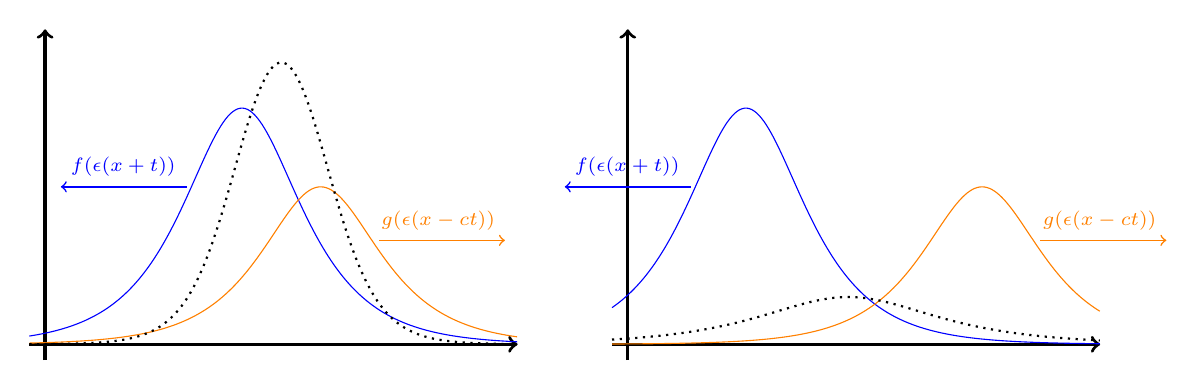
\begin{tikzpicture}[
	scale=2,
	declare function={sech(\x) = 2/(exp(\x) + exp(-\x));
					  fun1(\x,\c) = 1.5 * sech((\x-\c)*3;
					  fun2(\x,\c) = sech((\x-\c)*3);
	},
	]
	%axis
    \draw[->, very thick] (-0.1,0) -- (3,0) {};
    \draw[->, very thick] (0,-0.1) -- (0,2) {};
    
    %functions
    \draw[domain=-.1:3, samples = 200, color=blue] plot (\x, {fun1(\x, 1.25)} );
    \draw[domain=-.1:3, samples = 200, color=orange] plot (\x, {fun2(\x, 1.75)} );
    \draw[domain=-.1:3, samples = 200, thick, dotted] plot (\x, {2* fun1(\x,1.25) * fun2(\x,1.75)});
    
    %arrows
    \draw[->,line width=0.20mm,color=blue] (.9, 1) -- (0.1,1) {} node[above right] {\scriptsize $f(\epsilon(x+t))$};
    \draw[->,line width=0.20mm,color=orange] (2.12, .66) -- (2.92,.66) {} node[above left] {\scriptsize $g(\epsilon(x-ct))$};
    
    \begin{scope}[xshift=3.7cm]
	%axis
	\draw[->, very thick] (-0.1,0) -- (3,0) {};
	\draw[->, very thick] (0,-0.1) -- (0,2) {};
	
	%functions
	\draw[domain=-.1:3, samples = 200, color=blue] plot (\x, {fun1(\x, .75)} );
	\draw[domain=-.1:3, samples = 200, color=orange] plot (\x, {fun2(\x, 2.25)} );
	\draw[domain=-.1:3, samples = 200, thick, dotted] plot (\x, {0.3 * sech((\x - 1.4)*2});
	
	%arrows
	\draw[->,line width=0.20mm,color=blue] (.4, 1) -- (-0.4,1) {} node[above right] {\scriptsize $f(\epsilon(x+t))$};
	\draw[->,line width=0.20mm,color=orange] (2.62, .66) -- (3.42,.66) {} node[above left] {\scriptsize $g(\epsilon(x-ct))$};
    \end{scope}
\end{tikzpicture}
\caption{\label{fig-counter-propogating-interaction} The function \(f(\epsilon(x+t)) -f_\infty\) (shown in blue) moves to the left while \(g(\epsilon(x-ct))\) (shown in orange) moves to the right. Since they are localized, the product (shown by the dotted line) will quickly decay in time.}
\end{figure}

\begin{prop}
	Fix \(T_0> 0\) and suppose that \(f \in C([-T_0,T_0], \mcX_2^{k+1}(\R))\) and \(g \in C([-T_0,T_0], H^{k+1}_2(\R)) \), with \(k>2\) an integer. Also, suppose that \(f(X,T)\to f_\infty\) as \(X\to \infty\) for any \(T\in[-T_0,T_0]\). Then there exists a constant \(C>0\) such that 
	\begin{equation}\label{phi-bound}
		\sup_{t\in[-\epsilon^{-3}T_0,\epsilon^{-3}T_0]} \|\phi(\cdot,\epsilon t)\|_{H^k} \leq C \Bigg( \sup_{t\in[-\epsilon^{-3}T_0,\epsilon^{-3}T_0]} \left\{\| f(\cdot, \epsilon^3t) \|_{\mathcal X^{k+1}_{2}},  \| g(\cdot, \epsilon^3t) \|_{H^{k+1}_2} \right\}\Bigg)^3
	\end{equation}
	and
	\begin{equation}\label{psi-bound}
		\sup_{t\in[-\epsilon^{-3}T_0,\epsilon^{-3}T_0]} \|\psi(\cdot,\epsilon t)\|_{H^{k-1}} \leq C \Bigg( \sup_{t\in[-\epsilon^{-3}T_0,\epsilon^{-3}T_0]} \left\{\| f(\cdot, \epsilon^3t) \|_{\mathcal X^{k+1}_{2}},  \| g(\cdot, \epsilon^3t) \|_{H^{k+1}_2} \right\}\Bigg)^3,
	\end{equation}
	where \(\psi = \partial_2 \phi\).
\end{prop}

\begin{proof}
	Set \(\partial_2 \phi = \psi\). Taking the Fourier transform \(\mathcal F\) on both sides of \cref{phi-pde} and writing the ODE as a first order system, we get that 
	\begin{equation}
	\begin{aligned}
		&\partial_2 \begin{bmatrix} \hat \phi(k,\tau) \\ \hat \psi(k,\tau) \end{bmatrix} = \begin{bmatrix}\hat \psi(k,\tau) \\ -k^2 \hat\phi(k,\tau) \end{bmatrix} \\ &+ \begin{bmatrix}
			0 \\   \frac 1 2 k^2 \mathcal F[ (f^2(\cdot+\tau),\epsilon^2\tau)-f_\infty^2)g(\cdot-c\tau,\epsilon^2\tau) +(f(\cdot+\tau,\epsilon^2\tau)-f_\infty)g^2(\cdot-c\tau,\epsilon^2\tau)](k)
		\end{bmatrix}.
	\end{aligned}
	\end{equation}
	The semigroup generated by the linear part can be computed explicitly. Putting the solution into variation of constants form with initial conditions set to zero gives
	\begin{equation}
	\begin{aligned}
		&\hat  \phi(k,T) = \frac 1 2 \int_0^Tk\sin(k(T-\tau)) \times\\
		&\quad\mathcal F[ (f^2(\cdot+\tau),\epsilon^2\tau)-f_\infty^2)g(\cdot-c\tau,\epsilon^2\tau) +(f(\cdot+\tau,\epsilon^2\tau)-f_\infty)g^2(\cdot-c\tau,\epsilon^2\tau)](k)\, d\tau
	\end{aligned}
	\end{equation}
	and 
	\begin{equation}\label{psi-fourier-transform}
	\begin{aligned}
		&\hat  \psi(k,T) = \frac 1 2 \int_0^Tk^2\cos(k(T-\tau)) \times\\
		&\quad\mathcal F[ (f^2(\cdot+\tau,\epsilon^2\tau)-f_\infty^2)g(\cdot-c\tau,\epsilon^2\tau) +(f(\cdot+\tau,\epsilon^2\tau)-f_\infty)g^2(\cdot-c\tau,\epsilon^2\tau)](k)\, d\tau
	\end{aligned}
	\end{equation}
	Hence we can get that 
	\begin{equation}\label{phi-sobolev-bound}
	\begin{aligned}
		&\|\phi(\cdot, T) \|_{H^k} \\
		&\quad\leq C \| \hat\phi(\cdot, T) \|_{H^0_k} \\
		&\quad\leq C \int_0^T \| \partial_1 ((f^2(\cdot+\tau)-f_\infty^2)g(\cdot-c\tau)) \|_{H^k} + \| \partial_1( (f(\cdot+\tau)-f_\infty)g^2(\cdot-c\tau)) \|_{H^k} \, \mathrm d \tau \\
		&\quad\leq C \int_0^T \| f(\cdot+\tau)\partial_1 f(\cdot + \tau)g(\cdot-c\tau) \|_{H^k} + \|(f^2(\cdot+\tau) -f_\infty^2) \partial_1 g(\cdot - c\tau) \|_{H^k}  \\
		&\qquad + \|\partial_1f(\cdot+\tau) g^2(\cdot - c\tau) \|_{H^k} + \| (f(\cdot + \tau) -f_\infty) \partial_1 g(\cdot - c\tau) \|_{H^k}\, \mathrm{d}\tau \\ 
		&\quad\leq C \int_0^T \sup_{x\in\R} \frac 1 {\langle x + \tau\rangle_+^2 \langle x - c\tau\rangle^2} \times \Bigg( \|f\|^2_{\mathcal X^{k+1}_{2}} \| g \|_{H^{k+1}_2} + \|f\|_{\mathcal X^{k+1}_{2}} \| g \|^2_{H^{k+1}_2} \Bigg) \, \mathrm d \tau, 
	\end{aligned}
	\end{equation}
	whence \cref{phi-bound} follows. The proof for \cref{psi-bound} is analogous.
\end{proof}

\section{Setup of Lattice Equations}

The scalar second-order differential equation \cref{fput-lattice-equations-strain-variables} with potential \(V\) given by \cref{truncated-potential} can be rewritten as the following first-order system:
\begin{equation}\label{first-order-lattice-eqns}
	\left\{\begin{aligned}\dot u _n &= q_{n+1} - q_n, \\
	\dot q_n &= u_n - u_{n-1} - \frac{1} 6 ( u_n^3 - u^3_{n-1}),\end{aligned} \right. \quad n \in \Z.
\end{equation}

We will now introduce the traveling wave ansatz for the system in \cref{first-order-lattice-eqns}, but we first must assume certain regularity and decay of \(f\) and \(g\).
\begin{assum}\label{assumption-1}
	Let \(f\) and \(g\) be solutions of \cref{f-mKdV,g-gKdV}, respectively. Assume that \[f\in C_b(\R, \mcX_2^6(\R)) \quad \text{ and } \quad g\in C_b(\R,H_2^6(\R)).\] Furthermore, assume that \(f\) has fixed limits in its spatial variable at \(\pm \infty\) given by \(f_{\pm \infty}\).
\end{assum}

The traveling wave ansatz for \(u_n\) and \(q_n\) is then given by
\begin{equation}\label{u-ansatz}
	u_n(t) = \epsilon f(\epsilon(n+t), \epsilon^3t) + \epsilon g(\epsilon(n-ct), \epsilon^3 t) + \epsilon^3 \phi(\epsilon n , \epsilon t) + \mcU_n(t)
\end{equation}
and 
\begin{equation}\label{q-ansatz}
	q_n(t) = \epsilon F(\epsilon(n+t), \epsilon^3 t) + \epsilon G(\epsilon(n-ct), \epsilon^3 t) + \epsilon^3 \Phi(\epsilon n, \epsilon t) - \epsilon F_{-\infty} + \mcQ_n(t).
\end{equation}
The wave speed \(c\) is again given by \cref{ansatz-wave-speed}. The functions \(F\), \(G\), an \(\Phi\) are chosen to minimize the remainder terms from plugging in the ansatz back into \cref{first-order-lattice-eqns} and are given explicitly below:
\begin{align}
	F &:= f - \frac{\epsilon} 2 \partial_1 f + \frac{\epsilon^2} 8 \partial_1^2 f - \frac{\epsilon^2}{12} f^3  - \frac{\epsilon^3}{48} \partial_1^3 f + \frac{\epsilon^3} 8 f^2 \partial_1 f\\
	G &:= - g + \frac{\epsilon}{2}\partial_1 g + \frac{\epsilon^2 f_\infty^2} 4  g + \frac{\epsilon^2}{12}(g^3 + 3f_\infty g^2) -\frac{ \epsilon^2} 8 \partial_1^2 g  + \frac{\epsilon^3}{48} \partial_1^3 g \\
	&\qquad - \frac{\epsilon^3}{24} \partial_1(g^3 + 3f_\infty g^2) - \frac{\epsilon^3 f_\infty^2} 8 \partial_1 g \nonumber \\
	\Phi &:=  \partial_1^{-1}\psi - \frac{\epsilon} 2 \psi.
\end{align}
Here \(\psi = \partial_2 \phi\) and \(\partial_1^{-1}\) is defined as a Fourier multiplier. That \(\partial_1^{-1}\psi\) is well-defined and in \(H^5(\R)\) follows from \cref{psi-fourier-transform}. Namely, we have that 
\begin{equation}
\begin{aligned}
	&\mcF[\partial_1^{-1} \psi(\cdot, T)](k) = (ik)^{-1} \hat\psi(k,T) \\
	&\quad = \frac{-i} 2 \int_0^T k \cos(k(T-\tau)) \times \\ &\quad \mcF[(f^2(\cdot+\tau,\epsilon^2\tau)-f_\infty^2)g(\cdot-c\tau,\epsilon^2\tau) +(f(\cdot+\tau,\epsilon^2\tau)-f_\infty)g^2(\cdot-c\tau,\epsilon^2\tau)](k) \, d\tau
\end{aligned}
\end{equation}
and (following the same calculations in \cref{phi-sobolev-bound}) 
\begin{equation}
	\| \partial_1^{-1}\psi(\cdot,T) \|_{H^5} \leq C \int_0^T \sup_{x\in\R} \frac 1 {\langle x + \tau\rangle_+^2 \langle x - c\tau\rangle^2} \times \Bigg( \|f\|^2_{\mathcal X^{6}_{2}} \| g \|_{H^{6}_2} + \|f\|_{\mathcal X^{6}_{2}} \| g \|^2_{H^{6}_2} \Bigg) \, \mathrm d \tau. 
\end{equation}\Cref{assumption-1} implies that \(F\) has fixed limits in its spatial variable at \(\pm \infty\) given by \(F_{\pm\infty} = f_{\pm\infty} -\frac{\epsilon^2}{12} f^3_{\pm\infty}\).

We want \(\mcU(t)\) and \(\mcQ(t)\) to be elements of \(\ell^2(\Z)\) (at least locally in time). However, to satisfy \(\mcQ(0)\in\ell^2(\Z)\) and \(\dot u_n(0) = q_{n+1}(0) - q_n(0)\), a compatibility condition must hold.
\begin{assum}\label{assumption-2}
	Assume that \[\sum_{n=-\infty}^\infty \dot u_n(0) = \epsilon F_{+\infty} - \epsilon F_{-\infty}.\]
\end{assum}
Note that if this did not hold, then \(\mcQ_n(0)\not\to 0\) as \(n\to\infty\) and \(\mcQ(0)\notin \ell^2(\Z)\). That \(\mcQ(0)_n \to 0\) as \(n\to-\infty\) follows directly from the ansatz. The introduction of the constant \(\epsilon F_{-\infty}\) in \cref{q-ansatz} does not affect the dynamics of \(q\) in \cref{first-order-lattice-eqns}

An equivalent set of equations to \cref{first-order-lattice-eqns} are given by
\begin{equation}\label{error-lattice-eqns}
	\left\{\begin{aligned}
			\dot{\mathcal U}_n(t) =& \, \mathcal Q_{n+1}(t) - \mathcal Q_n(t) +\ResnI \\
\dot{\mathcal Q}_n(t) =& \, \mathcal U_n(t) - \mathcal U_{n-1}(t)  \\
&\quad - \frac 1 2 (\epsilon f(\epsilon(n+t)) + \epsilon g(\epsilon(n-ct)) + \epsilon^3\phi(\epsilon n))^2 \mathcal U_{n}(t) \\
&\quad + \frac 12  (\epsilon f(\epsilon(n-1+t)) + \epsilon g(\epsilon(n-1-ct)) + \epsilon^3\phi(\epsilon (n-1)))^2 \mathcal U_{n-1}(t) \\
&\quad +\ResnII + \mathcal B_n(\epsilon f + \epsilon g + \epsilon^3 \phi,  \mathcal U) 
	\end{aligned} \right. \hspace{-0.5em}n\in\Z,
\end{equation}
where
\begin{equation}
\begin{aligned}
	\ResnI =& \epsilon F(\epsilon(n+1+t)) - \epsilon F(\epsilon(n+t)) \\
	&\quad + \epsilon G(\epsilon(n+1-c t) - \epsilon G(\epsilon(n-c t) + \epsilon^3 \Phi(\epsilon (n+1))   - \epsilon^3 \Phi(\epsilon n) \\
	&\quad - \epsilon^2 \partial_1 f(\epsilon(n+t)) - \epsilon^4 \partial_2
	f(\epsilon(n+t)) \\
	&\quad + \epsilon^2 c \partial_1 g(\epsilon(n-ct)) - \epsilon^4 \partial_2 g(\epsilon(n-ct)) - \epsilon^4 \partial_2 \phi(\epsilon n) ,
\end{aligned}
\end{equation}
\begin{equation}
\begin{aligned}
	\ResnII =& \epsilon f(\epsilon(n+t)) - \epsilon f(\epsilon(n-1+t)) \\
	&\quad+ \epsilon g(\epsilon(n-c t)) - \epsilon g(\epsilon(n-1-c t) + \epsilon^3 \phi(\epsilon n) - \epsilon^3 \phi(\epsilon (n-1)) \\
	&\quad - \epsilon^2 \partial_1 F(\epsilon(n+t)) - \epsilon^4 \partial_2
	F(\epsilon(n+t)) \\
	&\quad + \epsilon^2 c \partial_1 G(\epsilon(n-ct)) - \epsilon^4 \partial_2 G(\epsilon(n-ct)) - \epsilon^4 \partial_2 \Phi(\epsilon n) \\
	&\quad - \frac 1 6 \Big( (\epsilon f(\epsilon(n+t)) + \epsilon g(\epsilon(n-c t)) + \epsilon^3 \phi(\epsilon n))^3 \\
	&\hspace{6em} - (\epsilon f(\epsilon(n-1+t)) + \epsilon g(\epsilon(n-1-c t)) + \epsilon^3 \phi(\epsilon (n-1)))^3 \Big),
\end{aligned}
\end{equation}
and 
\begin{equation}
\begin{aligned}
	&\mathcal B_n(\epsilon f + \epsilon g + \epsilon^3 \phi, \mathcal U) \\
	&\quad= -\frac 1 6 \Big( 3(\epsilon f(\epsilon(n+t) + \epsilon g(\epsilon(n-ct)) + \epsilon^3 \phi(\epsilon n))  \mathcal U^2_n(t) \\
	&\quad \qquad - 3(\epsilon f(\epsilon(n-1+t) + \epsilon g(\epsilon(n-1-ct)) + \epsilon^3 \phi(\epsilon (n-1)))  \mathcal U^2_{n-1}(t) \\
	&\quad\qquad + \mathcal U_n^3(t)  - \mathcal U_{n-1}^3(t)\Big).
\end{aligned}
\end{equation}
The terms \(\mcU\) and \(\mcQ\) control the error associated with the ansatz in \cref{u-ansatz,q-ansatz}. Thus if these terms remain small in the \(\ell^2(\Z)\) norm, then the traveling wave ansatz will remain valid.

\section{Preparatory Estimates}
 
To control the dynamics of \(\mcU\) and \(\mcQ\), we need estimates of the residuals and the nonlinearity. We will frequently need to bound the \(\ell^2(\Z)\) of a term by the \(H^1(\R)\) norm of a function. To this end the following lemma proved in \cite{dumas2014justification} is useful.
\begin{lem}\label{h1-ell2-ineq}
	There exists \(C>0\) such that for all \(X \in H^1(\R)\) and \(\epsilon \in (0,1)\), \[\|x\|_{\ell^2} \leq C \epsilon^{-1/2} \|X\|_{H^1},\] where \(x_n := X(\epsilon n)\), \(n\in \mathbb Z\).
\end{lem}


%Proof residual terms and nonlinear terms remain small
\begin{lem}\label{residual-nonlinearity-bounds}
	Let \(f\) and \(g\) be solutions of \cref{f-mKdV,g-gKdV}, respectively, such that \(f\in C([-\tau_0, \tau_0] , \mcX^6_2)\) and \(g\in C([-\tau_0,\tau_0], H^6_2)\). Let \(\tau_0 > 0\) be fixed and \(\delta>0\) be as \begin{equation}\label{delta-defn}
		\delta := \max \left\{\sup_{\tau\in[-\tau_0, \tau_0]}\|f(\cdot,\tau)\|_{\mcX^6_2},\ \sup_{\tau\in[-\tau_0, \tau_0]} \|g(\cdot, \tau)\|_{H^6_2} \right\}
	\end{equation}
 	Then there exists a \(\delta\)-independent constant \(C>0\) such that the residual and nonlinear terms satisfy
	\begin{equation}\label{res-ineq}
		\| \ResI \|_{\ell^2} + \|\ResII \|_{\ell^2} \leq C \epsilon^{11/2} (\delta + \delta^5)
	\end{equation}
	and 
	\begin{equation}\label{nonlinear-ineq}
		\| \mathcal B_n(\epsilon f + \epsilon g + \epsilon^3 \phi, \mathcal U) \|_{\ell^2} \leq C\epsilon [ (\delta+\epsilon^2\delta^3) \|\mcU\|_{\ell^2} ^2 + \|\mcU\|_{\ell^2}^3]
	\end{equation}
	for every \(t\in[-\epsilon^{-3} \tau_0, \epsilon^{-3} \tau_0]\) and \(\epsilon \in (0,1).\)
\end{lem}

\begin{proof}
	We first focus on bounding \(\ResI\). Looking first at the terms in \(\ResI\) involving \(f\) and \(F\) and using Taylor expansions and \cref{f-mKdV}, we get the following:
	\begin{equation}\label{F-res1}
		\begin{aligned}
			&\epsilon F(\cdot + \epsilon) - \epsilon F - \epsilon^2 \partial_1 f - \epsilon^4 \partial_2 f = \\
			&\hspace{10em}\begin{aligned}
				&\epsilon^2 \partial_1 f + & & \frac{\epsilon^3} 2 \partial_1^2 f +& &\frac{\epsilon^4} 6 \partial_1^3 f   & + &\frac{\epsilon^5}{24} \partial_1^4 f  \\
				& & - &\frac{\epsilon^3} 2 \partial_1^2 f & - &\frac{\epsilon^4} 4 \partial_1^3 f & - & \frac{\epsilon^5} {12} \partial_1^4 f \\
				& & & & + &\frac {\epsilon^4} 8 \partial_1^3 f & + & \frac{\epsilon^5}{16} \partial_1^4 f   \\
				& & & & - &\frac {\epsilon^4} {12} \partial_1 (f^3) & - & \frac{\epsilon^5}{24} \partial_1^2(f^3)\\
				& & & & & & - & \frac{\epsilon^5}{48} \partial_1^4 f \\
				& & & & & & + & \frac{\epsilon^5}{24} \partial_1^2 (f^3) \\
				-&\epsilon^2 \partial_1 f \\
				& & & & + &\frac{\epsilon^4}{12}\partial_1(f^3) \\
				& & & & - &\frac{\epsilon^4}{24}\partial^3 f & & & + I_{f,1}(n,t),
			\end{aligned}
		\end{aligned}
	\end{equation}
	where \(I_{f,1}\) contains the integral remainder terms:
	\begin{equation}\label{If1}
	\begin{aligned}
		I_{f,1}(n,t) := \ &\frac{\epsilon^6} {24} \int_0^1 \partial_1^5 f(\epsilon(n+t+s))(1-s)^4\, ds - \frac{\epsilon^6} {12} \int_0^1 \partial_1^5 f(\epsilon(n+t+s))(1-s)^3\, ds \\
		+ & \frac{\epsilon^6} {16} \int_0^1 \partial_1^5 f(\epsilon(n+t+s))(1-s)^2\, ds -  \frac{\epsilon^6} {24} \int_0^1 \partial_1^3 (f^3)(\epsilon(n+t+s))(1-s)^2\, ds \\
		- & \frac{\epsilon^6}{48} \int_0^1 \partial_1^5f(\epsilon(n+t+s))(1-s)\, ds +  \frac{\epsilon^6}{24} \int_0^1 \partial_1^3 (f^3)(\epsilon(n+t+s)) (1-s)\, ds.
	\end{aligned}
	\end{equation}
	Note that the terms involving lower orders of \(\epsilon\) cancel, and so we are only left with \(I_{f,1}\) which is of order \(\epsilon^6\). Applying \cref{h1-ell2-ineq} (and \cref{prod-rule-1-lem,prod-rule-2-lem} when needed) to the terms in \cref{If1} gives that the \(\ell^2\) norm on the left-hand side of the above inequality can be bounded by \[C(\epsilon^{11/2}(\delta + \delta^3))\] for some choice of constant \(C>0\).
	
	Doing the same Taylor expansion for the \(g\) and \(G\) gives
	\begin{equation}
		\begin{aligned}
			&\epsilon G(\cdot + \epsilon) - \epsilon G + \epsilon^2c \partial_1 g - \epsilon^4 \partial_2 g  = \\
			&\hspace{10em}\begin{aligned}
				- & \epsilon^2 \partial_1 g & -&\frac{\epsilon^3} 2 \partial_1^2 g & - &\frac{\epsilon^4} 6 \partial_1^3 g & - & \frac{\epsilon^5}{24} \partial_1^4 g \\
				& & +&\frac{\epsilon^3} 2 \partial_1^2 g & + &\frac{\epsilon^4} 4\partial_1^3 g &+ & \frac{\epsilon^5}{12} \partial_1^4 g \\
				& & & & + &\frac{\epsilon^4 f_\infty^2} 4\partial_1 g & + & \frac{\epsilon^5f_\infty^2} 8 \partial_1^2 g  \\
				& & & & + &\frac{\epsilon^4} {12}\partial_1 (g^3) & + & \frac{\epsilon^5}{24} \partial_1^2(g^3) \\
				& & & & + &\frac{\epsilon^4} {12}\partial_1 (3f_\infty g^2) & + & \frac{\epsilon^5}{24}\partial_1^2(3f_\infty g^2)  \\
				& & & & - &\frac{\epsilon^4} {8}\partial_1^3 g & - &  \frac{\epsilon^5}{16} \partial_1^4 g  \\ 
				& & & & & & + & \frac{\epsilon^5}{48} \partial_1^4 g  \\
				& & & & & & - & \frac{\epsilon^5}{24} \partial_1^2(g^3) \\
				& & & & & & - & \frac{\epsilon^5}{24} \partial_1^2(3f_\infty g^2) \\
				& & & & & & - & \frac{\epsilon^5 f_\infty ^2} 8 \partial_1^2 g  \\
				+&\epsilon^2 \partial_1g \\
				& & & & - & \frac{\epsilon^4f_\infty ^2}{4} \partial_1 g \\
				& & & & - &\frac{\epsilon^4} {12}\partial_1 (g^3) \\
				& & & & - &\frac{\epsilon^4} {12}\partial_1 (3f_\infty g^2) \\ 
				& & & & + & \frac{\epsilon^4}{24} \partial_1^3 g && &+ I_{g,1}(nt),
			\end{aligned}
		\end{aligned}
	\end{equation}
	where \(I_{g,1}\) contains the integral remainder terms.
	\begin{equation}\label{Ig1}
	\begin{aligned}
		&I_{g,1}(n,t) := \\
		-&\frac{\epsilon^6} {24} \int_0^1 \partial_1^5 g(\epsilon(n - ct + s)) (1-s)^4 \, ds +\frac{\epsilon^6} {12} \int_0^1 \partial_1^5 g(\epsilon(n - ct + s)) (1-s)^3 \, ds \\
		+&\frac{\epsilon^6 f_\infty^2} 8 \int_0^1 \partial_1^3 g(\epsilon(n - ct + s)) (1-s)^2 \, ds +\frac{\epsilon^6} {24} \int_0^1 \partial_1^3(g^3)(\epsilon(n - ct + s)) (1-s)^2 \, ds \\
		+&\frac{\epsilon^6} {24} \int_0^1 \partial_1^3(3f_\infty g^2)(\epsilon(n - ct + s)) (1-s)^2 \, ds - \frac{\epsilon^6} {16} \int_0^1 \partial_1^5g(\epsilon(n - ct + s)) (1-s)^2 \, ds \\
		+ & \frac{\epsilon^6}{48}\int_0^1 \partial_1^5 g(\epsilon(n-ct+s))(1-s)\, ds -  \frac{\epsilon^6}{24} \int_0^1 \partial_1^3(g^3)(\epsilon(n-ct+s))(1-s)\, ds \\
		- & \frac{\epsilon^6}{24} \int_0^1 \partial_1^3(3f_\infty g^2)(\epsilon(n-ct+s))(1-s)\, ds - \frac{\epsilon^6f_\infty ^2}{8} \int_0^1 \partial_1^3 g(\epsilon(n-ct+s)) (1-s) \, ds
	\end{aligned}
	\end{equation}
	All terms except those of order \(\epsilon^6\) cancel and the terms in \cref{Ig1} can be controlled by \cref{h1-ell2-ineq}. 

	
	Similarly we have
	\begin{equation}
		\epsilon^3 \Phi(\epsilon(n+1), \epsilon t) - \epsilon^3\Phi(\epsilon n , \epsilon t) - \epsilon^4 \partial_2 \phi_2(\epsilon n, \epsilon t) =  \frac{\epsilon^6} 2 \int_0^1 \partial_1^2 \psi(\epsilon(n+s),\epsilon t)(1-s)^2\, ds,
	\end{equation}
	whose \(\ell^2\) norm can also be controlled.
	
	Therefore we have 
	\begin{equation}
		\| \ResI \|_{\ell^2} \leq C \epsilon^{11/2}(\delta + \delta^3)
	\end{equation}

	The bound on \(\ResII\) can be approached similarly. Focusing first on the terms with \(f\) and \(F\) in \(\ResII\), we have that all terms of order \(\epsilon^5\) or lower cancel. We are again left with \(\epsilon^6\) order terms that are integral remainders from Taylor expansion that are controlled and a term of the form 
	\begin{equation}
		\partial_2\left(\frac{1} 8 \partial_1^2 f - \frac{1}{12} f^3  - \frac{\epsilon}{48} \partial_1^3 f + \frac{\epsilon} 8 f^2 \partial_1 f\right),
	\end{equation}
  	which can also be controlled by using the PDE for \(f\) \cref{f-mKdV} to get rid of the derivatives in time and then using \cref{h1-ell2-ineq}.
  	
  
	\begin{equation}
		\begin{aligned}
			&\epsilon f(\cdot) - \epsilon f(\cdot - \epsilon) - \epsilon^2 \partial_1 F -\epsilon^4\partial_2 F - \frac{\epsilon^3} 6 (f^3(\cdot) - f^3(\cdot - \epsilon)) =\\
			&\quad \begin{aligned}
				&\epsilon^2\partial_1 f &- &\frac{\epsilon^3} 2 \partial_1 f &+ &\frac{\epsilon^4} 6 \partial_1^3f & - & \frac{\epsilon^5}{24} \partial_1^4 f\\
				-&\epsilon^2\partial_1 f & + & \frac{\epsilon^3} 2 \partial_1^2 f &+& \frac{\epsilon^4}{12} \partial_1(f^3) - \frac{\epsilon^4} 8 \partial_1^3 f & + &  \frac{\epsilon^5}{48} \partial_1^4 f - \frac{\epsilon^5}{24}\partial_1^2(f^3)\\
				&&&& -&\epsilon^4 \partial_2 f & + & \frac{\epsilon^5} 2 \partial_1 \partial_2 f\\
				&&&& -&\frac{\epsilon^4} 6 \partial_1(f^3) & + & \frac{\epsilon^5}{12} \partial_1(f^3) & &+ I_{f,2}(n,t).
			\end{aligned}
		\end{aligned}
	\end{equation}
	\begin{equation}
	\begin{aligned}
		I_{f,2}(n,t) := - & \frac{\epsilon^6} {24} \int_{-1}^0 \partial_1^5 f (\epsilon(n+t+s))(s+1)^4\, ds \\
		+ & \frac{\epsilon^6} {12} \int_{-1}^0 \partial_1^2(f^3)(\epsilon(n+t+s))(s+1)^2\, ds \\
		+ & \epsilon^6\partial_2\left(\frac{1} 8 \partial_1^2 f - \frac{1}{12} f^3  - \frac{\epsilon}{48} \partial_1^3 f + \frac{\epsilon} 8 f^2 \partial_1 f\right)
	\end{aligned}
	\end{equation}
	All the above terms except the for those of order \(\epsilon^6\).


	\begin{equation}
	\begin{aligned}
			&\epsilon^2 \partial_1 g & - & \frac{\epsilon^3} 2 \partial_1^2g & + & \frac{\epsilon^4} 6 \partial_1^3 g & - & \frac{\epsilon^5}{24} \partial_1^4 g  \\
			&&&&+&\epsilon^4 \partial_1 \phi & - & \frac{\epsilon^5} 2 \partial_1^2  \phi \\
			-&\epsilon^2\partial_1 g & + & \frac{\epsilon^3} 2 \partial_1^2 g & - & \frac{\epsilon^4} 8 \partial_1^3 g  + \frac{\epsilon^4 L^2} 4 \partial_1 g & + & \frac{\epsilon^5}{48} \partial_1^4 g \\
			&&&&+ & \frac{\epsilon^4}{12} \partial_1(g^3 + 3Lg^2) & - & \frac{\epsilon^5}{24} \partial_1^2(g^3 + 3Lg^2)\\
			&&&&&& - & \frac{\epsilon^5L^2} 8 \partial_1^2 g \\
			&&&&+&\frac{\epsilon^4L^2} 4 \partial_1g  & - & \frac{\epsilon^5L^2} 8 \partial_1^2 g \\
			&&&& +&\epsilon^4 \partial_2 g & - & \frac{\epsilon^5} 2 \partial_1 \partial_2 g \\ 
			&&&&-&\epsilon^4 \partial_2 \partial_1^{-1} \psi & + & \frac{\epsilon^5} 2 \partial_2 \psi\\
			&&&&-&\frac{\epsilon^4} 6 \partial_1(g^3 + 3g^2 f + 3gf^2) & + & \frac{\epsilon^5}{12}\partial_1^2(g^3 + 3g^2 f + 3gf^2)
	\end{aligned}
	\end{equation} 

	\begin{equation}
	\begin{aligned}
		&I_{g,2}(n,t) = \\
		- & \frac{\epsilon^6} {24} \int_{0}^1 \partial_1^5 g(\epsilon(n-s-ct))  (s-1)^4 \, ds -  \frac{\epsilon^6}2 \int_{-1}^0\cdots \, ds \\
		- & \frac{\epsilon^6 f_\infty^2}{4}\partial_1\left( \frac{f_\infty^2} 4  g + \frac{1}{12}(g^3 + 3f_\infty g^2) -\frac{ 1} 8 \partial_1^2 g  + \frac{\epsilon}{48} \partial_1^3 g - \frac{\epsilon}{24} \partial_1(g^3 + 3f_\infty g^2) - \frac{\epsilon f_\infty^2} 8 \partial_1 g\right) \\
		-&  \epsilon^6\partial_2\left( \frac{f_\infty^2} 4  g + \frac{1}{12}(g^3 + 3f_\infty g^2) -\frac{ 1} 8 \partial_1^2 g  + \frac{\epsilon}{48} \partial_1^3 g - \frac{\epsilon}{24} \partial_1(g^3 + 3f_\infty g^2) - \frac{\epsilon f_\infty^2} 8 \partial_1 g\right) \\
		+ & \frac{\epsilon^6} {12} \int_{-1}^0 \cdots ds 
	\end{aligned}
	\end{equation}
	
	%\epsilon^6\partial_2(G_2+ \epsilon G_3)
	%\frac{\epsilon^6 L^2}{4}\partial_1(G_2 + \epsilon G_3)
	For the remaining terms, we have that terms of order \(\epsilon^3\) or lower cancel out. The terms of order \(\epsilon^4\) are equal to 
	\begin{equation}
		-\partial_2 \partial_1^{-1} \psi+ \partial_1 \phi  - \frac 1 6 \partial_1(3(f^2 - f_\infty^2) g + 3(f-f_\infty) g^2).
	\end{equation}
	Formally applying \(\partial_1\) implies that the above terms should be constant in space (taking a derivative with respect to the rescaled \(\epsilon x = \epsilon n\) shows that this is the case). Since all the terms decay to zero at spatial infinity, they are exactly zero.
	
	The terms of order \(\epsilon^5\) can be rewritten as
	\begin{equation}
		\frac 1 4 \partial_1( - 2 \partial_2 g - \frac 1 {12} \partial_1^3 g + \frac 1 6 (g^3 + 3f_\infty g^2)) + \frac 1 2 (\partial_2^2\phi - \partial_1^2\phi + \frac 1 6 \partial_1^2(3(f-f_\infty )g^2 + 3 (f^2-f_\infty^2)g))
	\end{equation}
	which is equal to zero. The remaining terms are all of order of \(\epsilon^6\) or above are integral remainders from Taylor expansion and terms of the form 
	\begin{equation}
		\partial_2(G_2+ \epsilon G_3) \quad \text{and} \quad f_\infty^2 \partial_1(G_2 + \epsilon G_3).
	\end{equation}
	We can the get the following bound: \[\| \mathrm{Res}^{(2)}(t) \|_{\ell^2} \leq C \epsilon^{11/2} (\delta + \delta^5).\] Interpolating between powers of \(\delta\) gives the desired inequality \cref{res-ineq}.
	
	The proof of \cref{nonlinear-ineq} follows immediately.
\end{proof}

%Show energy is coercive and its derivative remains bounded

Define 
\begin{equation}\label{energy-function}
	\mathcal E(t) = \frac 1 2 \sum_{n\in \mathbb Z} \mathcal Q_n^2(t) + \mathcal U_n^2(t) - \frac 1 2 \left(\epsilon f(\epsilon(n+t), \epsilon^3 t) + \epsilon g(\epsilon(n-ct, \epsilon^3t) + \epsilon^3 \phi(\epsilon n, \epsilon t)\right)^2 \mathcal U_n^2(t)
\end{equation}
\begin{lem}\label{energy-coercive-bounds-lem}
	Fix \(\tau_0>0 \) and let \(\delta\) be given by \cref{delta-defn} . There exists \(\epsilon_0 = \epsilon_0(\delta) >0\) sufficiently small such that for every \(\epsilon \in (0,\epsilon_0)\) and for every local solution \((\mathcal U, \mathcal Q) \in C^1([-\tau_0\epsilon^{-3}, \tau_0\epsilon^{-3}], \ell^2(\mathbb Z))\) of \cref{error-lattice-eqns}, the energy-type quantity given in \cref{energy-function} is coercive with the bound
	\begin{equation}\label{coercive-bound}
		\|\mathcal Q(t) \|_{\ell^2}^2 + \| \mathcal U (t) \|_{\ell^2}^2 \leq  4 \mathcal E(t), \quad \text{for } t\in(-\tau_0\epsilon^{-3}, \tau_0\epsilon^{-3}).
	\end{equation}
	Moreover, there exists \(C> 0\) independent of \(\epsilon\) and \(\delta\) such that 
	\begin{equation}
		\left|\frac{d\mathcal E}{dt} \right| \leq C \mathcal E^{1/2}\left[ \epsilon^{11/2} (\delta + \delta^5)  + \epsilon^3\delta^2\mathcal E^{1/2} + \epsilon(\delta + \mathcal{E}^{1/2})\mathcal E\right]
	\end{equation}
	for every \(t\in [-\tau_0\epsilon^{-3}, \tau_0\epsilon^{-3}]\) and \(\epsilon \in (0,\epsilon_0)\). 	  
\end{lem}
\begin{proof}
	Note that \(\delta>0\) can be used to control the \(L^\infty(\R)\) norms of \(f\), \(g\), and \(\psi\). Thus we can choose \(\epsilon_0\) small enough so that for \(\epsilon \in (0,\epsilon_0)\) we have 
	\begin{equation}
		1 - \frac 12 \left( \epsilon \| f\|_{L^\infty} + \epsilon \|g\|_{L^\infty} + \epsilon^3 \| \phi \|_{L^\infty} \right)^2 \geq \frac 12,
	\end{equation}
	independent on the particular choices of \(f\) and \(g\). 	Hence
	\begin{equation}
		\mathcal E(t) \geq \frac 1 2 \| \mathcal Q \|_{\ell^2}^2 + \frac 1 4 \| \mathcal U\|_{\ell^2}^2 \geq \frac 1 4\| \mathcal Q \|_{\ell^2}^2 + \frac 1 4 \| \mathcal U\|_{\ell^2}^2
	\end{equation}
	and \cref{coercive-bound} follows.
	
	Now we take the time derivative of \(\mathcal E\) to get that 
	\begin{equation}
	\begin{aligned}
		\frac{d\mathcal E}{dt} = \sum_{n \in \Z} &\mathcal Q_n(t) \ResnII + \mathcal Q_n(t) 	\mathcal B_n(\epsilon f + \epsilon g + \epsilon^3 \phi, \mathcal U(t) \\
		&+ \mathcal U_n(t) \ResnI \left( 1 - \frac 12 (\epsilon f+ \epsilon g + \epsilon^3 \phi)^2  \right) \\
		&+ \mathcal U_n^2(t)(\epsilon f + \epsilon g + \epsilon^3 \phi) \times (\epsilon^2\partial_1 f + \epsilon^4\partial_2 f -\epsilon^2 c \partial_1 g + \epsilon^4 \partial_2 g + \epsilon^4 \partial_2 \phi).
	\end{aligned}
	\end{equation}
	Then using the Cauchy inequality, taking \(\ell^\infty\) norms, and applying \cref{res-ineq,nonlinear-ineq}, we get that
	\begin{equation}
	\begin{aligned}
		\left| \frac{d\mathcal E}{dt} \right| \leq& \| \mathcal Q \|_{\ell^2 }\times \|\ResII \|_{\ell^2} + \| \mathcal Q \|_{\ell^2} \times \| \mathcal B \|_{\ell^2}  + \|\mathcal U \|_{\ell^2} \times \| \ResnI \|_{\ell^2}\\
		&\quad + \|\mathcal U \|_{\ell^2}^2 \times  (\epsilon\delta + \epsilon \delta + \epsilon^3 \delta^3)\times (\epsilon^2\delta + \epsilon^4\delta + \epsilon^2 c \delta + \epsilon^4 \delta + \epsilon^4 \delta^3) \\
		\leq& C\Big[\mathcal E^{1/2} \epsilon^{11/2}(\delta + \delta^5) + \mathcal E^{1/2}\epsilon [(\delta + \epsilon^2 \delta^3)\mathcal E + \mathcal E^{3/2}]  \\
		&\quad + \mathcal E(\epsilon^3 \delta^2 + \epsilon^5\delta^2 + \epsilon^5 \delta^4 + \epsilon^7\delta^4 + \epsilon^7 \delta^6) \Big],
	\end{aligned}
	\end{equation}
	with \(C>0\) independent of \(\epsilon\) and \(\delta\). The right-hand side of the above inequality can be simplified by taking \(\epsilon_0\) smaller. That is, taking \(\epsilon_0\) sufficiently small (dependent on \(\delta\)), we can absorb higher orders of \(\epsilon\) into lower orders. For example, \(\epsilon^3 \delta^2 + \epsilon^5\delta^2 \leq 2 \epsilon^3 \delta^2\) for \(\epsilon\) small enough. Thus we arrive at  		
	\begin{equation}
		\left|\frac{d\mathcal E}{dt} \right| \leq C \mathcal E^{1/2}\left[ \epsilon^{11/2} (\delta + \delta^5)  + \epsilon^3\delta^2\mathcal E^{1/2} + \epsilon(\delta + \mathcal{E}^{1/2})\mathcal E\right]
	\end{equation}
	as desired.
\end{proof}


Lastly, before we can prove our main result, we must show that for appropriate initial conditions that \(\mcU(0)\) and \(\mcQ(0)\) are suitably small. In particular, we want our initial conditions to be ``close to" the traveling wave ansatz in the sense that 
\begin{equation}
	u_n(0) \approx \epsilon f(\epsilon n , 0) + \epsilon g(\epsilon n , 0)
\end{equation}
and 
\begin{equation}
	\dot u_n(0) \approx \epsilon \partial_1 f(\epsilon n , 0) -\epsilon^2 g(\epsilon n,0)
\end{equation}
where the higher-order \(\epsilon\) terms are neglected. Recall that we assume \(\phi\) and \(\partial_1\phi\) to have initial conditions exactly equal to zero, so those terms drop. A seemingly appropriate notion of ``closeness" would be in the \(\ell^2\) norm, as used in \cite{khan2017long,schneider2000counter}. However, since \(q_n(0) = \sum_{k=-\infty}^{n-1} \dot u_{k}(0)\), we may lose some decay due to the summation and \(\mcQ(0)\) will not be in \(\ell^2\). To counter this, we need some extra localization assumptions on \(\dot u_n(0)\).

\begin{assum}\label{assumption-3}
	Suppose that the initial conditions for \(u\) satisfy
	\begin{equation}
		\| u(0) - \epsilon f(\epsilon \cdot, 0) - \epsilon g(\epsilon \cdot, 0) \|_{\ell^2} + \| \dot u(0) - \epsilon^2 \partial_1 f(\epsilon \cdot, 0) + \epsilon^2 \partial g (\epsilon \cdot , 0) \|_{\ell^2_2} \leq \epsilon^{5/2}
	\end{equation}
	and that \(f(\cdot, 0) \in \mcX^6_2\) and \(g(\cdot, 0) \in H^6_2\)
\end{assum}

The \(\ell^2_2\) norm will be sufficient to get that the summation is in \(\ell^2\) based on the following lemma.
\begin{restatable}{lem}{elltwo}
\label{ell22-lemma}
	If \(a\in \ell^2_2(\Z)\) and 
	\begin{equation}
		\sum_{k=-\infty}^n a_k = 0,
	\end{equation}
	then \(b_n = \sum_{k=-\infty}^n a_k\) is in \(\ell^2(\Z)\) and 
	\begin{equation}
		\|b\|_{\ell^2} \leq C \|a\|_{\ell^2_2}
	\end{equation}
	for some \(C> 0\) independent of \(a\).
\end{restatable} 
See \cref{lemma-appendix} for proof.


We can now show the following.
\begin{lem}\label{initial-conditions-lem}
	Let \cref{assumption-2,assumption-3} hold. Then \(\mcU(0),\mcQ(0) \in \ell^2(\Z)\) satisfy
	\begin{equation}\label{diff-eqn}
		\dot u_n(0) = q_{n+1}(0) - q_n(0)
	\end{equation}
	and 
	\begin{equation}\label{initial-condition-ineq}
		\| \mcU(0) \|_{\ell^2} + \|\mcQ(0)\|_{\ell^2} \leq C \epsilon^{5/2}
	\end{equation}
	with \(C>0\) independent of \(\epsilon\).
\end{lem}

\begin{proof}
	That \(\|\mcU(0)\|_{\ell^2}\leq C \epsilon^{5/2}\) follows immediately from applying \cref{assumption-3} to \cref{u-ansatz}.
	
	For \(q_n(0)\) to satisfy \cref{diff-eqn}, it must equal \(\sum_{k=-\infty}^{n-1} \dot u_k(0)\) (modulo a constant which we assume without loss of generality to be zero). Thus we have
	\begin{equation}\label{q0-summation}
	\begin{aligned}	
		q_n(0) =& \sum_{k=-\infty}^{n-1} \dot u_n(0)\\
		=& \sum_{k=-\infty}^{n-1}\left[ \dot u_k(0) - \epsilon^2 \partial_1 f(\epsilon k,0) - \epsilon^4 \partial_1 f(\epsilon k,0) + \epsilon^2 c \partial_1 g(\epsilon k,0) - \epsilon^4 \partial_2g(\epsilon k,0)\right] \\
		&+\sum_{k=-\infty}^{n-1}\left[  \epsilon^2 \partial_1 f(\epsilon k,0) +\epsilon^4 \partial_1 f(\epsilon k,0) - \epsilon F(\epsilon(k+1),0) +\epsilon F(\epsilon k ,0)  \right] \\
		&+ \sum_{k=-\infty}^{n-1}\left[ - \epsilon^2 c\partial_1 g(\epsilon k,0) +\epsilon^4 \partial_1 g(\epsilon k,0) - \epsilon G(\epsilon(k+1),0) +\epsilon G(\epsilon k ,0)  \right] \\
		&+ \epsilon F(\epsilon n, 0) - \epsilon F_{-\infty} + \epsilon G(\epsilon n, 0).
	\end{aligned}
	\end{equation}
	Comparing \cref{q0-summation} to \cref{q-ansatz}, we have that 
	 \begin{equation}\label{mcq-zero}
	 \begin{aligned}
		\mcQ_n(0) =& \sum_{k=-\infty}^{n-1}\left[ \dot u_k(0) - \epsilon^2 \partial_1 f(\epsilon k,0) - \epsilon^4 \partial_1 f(\epsilon k,0) + \epsilon^2 c \partial_1 g(\epsilon k,0) - \epsilon^4 \partial_2g(\epsilon k,0)\right] \\
		&+\sum_{k=-\infty}^{n-1}\left[  \epsilon^2 \partial_1 f(\epsilon k,0) +\epsilon^4 \partial_1 f(\epsilon k,0) - \epsilon F(\epsilon(k+1),0) +\epsilon F(\epsilon k ,0)  \right] \\
		&+ \sum_{k=-\infty}^{n-1}\left[ - \epsilon^2 c\partial_1 g(\epsilon k,0) +\epsilon^4 \partial_1 g(\epsilon k,0) - \epsilon G(\epsilon(k+1),0) +\epsilon G(\epsilon k ,0)  \right].
	\end{aligned}
	\end{equation}
	That \(\mcQ_n(0)\to 0\) as \(n\to\infty\) is guaranteed by \cref{assumption-2}. Now \cref{ell22-lemma} can be applied to get the result if the summands are in \(\ell^2_2\) and of order \(\epsilon^{5/2}\). The first summand satisfies this condition because of \cref{assumption-3}. The latter summands also satisfy this condition based on earlier calculations on the residuals. For example, referencing \cref{F-res1}, the second summand is equal to a sum of integral terms of the form
	\begin{equation}
		\frac{\epsilon^6}{24} \int_0^1 \partial_1^5 f(\epsilon(n+s), 0)(1-s)^4\, ds
	\end{equation}
	which are elements of \(\ell^2_2\) (since \(f(\cdot, 0) \in \mcX_2^6\)) and are of order \(\epsilon^{5/2}\). A similar conclusion holds for the third summand relying on \(g\in H^6_2\).
	
	Thus we have \cref{initial-condition-ineq} where the \(C>0\) can be chosen based on the norms of \(f\) and \(g\).
\end{proof}
\section{Proof of Long-Time Stability}

Now with the setup complete, the main result of this chapter can be shown. The result and proof are analogous to those of \cite[Thm.~1]{khan2017long}.

\begin{theorem}
	Let \cref{assumption-1} hold and set 
	\begin{equation}
		\delta = \max \left\{\sup_{\tau\in\R}\|f(\cdot,\tau)\|_{\mcX^6_2},\ \sup_{\tau\in \R} \|g(\cdot, \tau)\|_{H^6_2} \right\}
	\end{equation}
	For fixed \(r\in(0,1/2)\), there exists positive constants \(\epsilon_0\), \(C\), and \(K\) such that for all \(\epsilon \in(0,\epsilon_0)\), when initial data \((u(0), \dot u(0))\) satisfy \cref{assumption-2,assumption-3}, the unique solution \((u,q)\) to the FPU equation \cref{first-order-lattice-eqns} belongs to 
	\begin{equation}
		C^1([-t_0(\epsilon), t_0(\epsilon)], \ell^\infty(\mathbb Z))
	\end{equation}
	with \(t_0(\epsilon):= r K^{-1} \epsilon^{-3} | \log (\epsilon) | \) and satisfies
	\begin{equation}
	\begin{aligned}
		&\| u(t) - \epsilon f(\epsilon(\cdot+t), \epsilon^3 t) -\epsilon g(\epsilon(\cdot -ct) ,\epsilon^3 t) \|_{\ell^2} \\
		&\quad + \| \dot u(t) - \epsilon \partial_1 f(\epsilon (\cdot +t),\epsilon^3t)  +\epsilon^2 \partial_1 g(\epsilon(\cdot - ct), \epsilon^3t)\|_{\ell^2} \leq C \epsilon^{5/2 - r}, \quad t\in[-t_0(\epsilon), t_0(\epsilon)].
	\end{aligned}
	\end{equation}
\end{theorem}

\begin{proof}
	%Need to show local existence of solutions
	
	Set \(\mathcal S := \mathcal E ^{1/2}\) where \(\mathcal E\) is defined in \cref{energy-function}. From the results in \cref{initial-conditions-lem}, we get that \(\mathcal S(0) \leq C_0 \epsilon^{5/2}\) for some constant \(C_0 > 0\) and \(\epsilon_0\) as chosen in \cref{energy-coercive-bounds-lem}. For fixed constants \(r\in(0,1/2)\), \(C> C_0\), and \(K > 0\), define the maximal continuation time by 
	\begin{equation}
		T_{C,K,r} := \sup \left\{T_0 \in (0, r K^{-1} \epsilon^{-3} |\log(\epsilon)|]: \mathcal S(t) \leq C \epsilon^{5/2 -r}, t\in [-T_0, T_0]\right\}.
	\end{equation} 
	We also define the maximal evolution time of the mKdV equation as \(\tau_0(\epsilon) = rK^{-1}|\log(\epsilon)|\). The goal is then to pick \(C\) and \(K\) so that \(T_{C,K,r} = \epsilon^{-3} \tau_0(\epsilon)\).
	
	We have that
	\begin{equation}
	\begin{aligned}
		\left | \frac d {dt} \mathcal S(t) \right | &= \frac 1 {2 \mathcal E ^{1/2}} \left | \frac d {dt} \mathcal E(t) \right| \\
		&\leq C_1(\delta + \delta^5) \epsilon^{11/2} + C_2 \epsilon^3\left[ \delta^2 + \epsilon^{-2}(\delta + \mathcal S) \mathcal S \right]\mathcal S
	\end{aligned}
	\end{equation}
	where \(C_1, C_2 > 0\) are independent of \(\delta\) and \(\epsilon\). While \(|t| \leq T_{C,K,r}\),
	\begin{equation}
		C_2 \left[ \delta^2 + \epsilon^{-2}(\delta + \mathcal S) \mathcal S \right] \leq C_2 \left[ \delta^2  + \epsilon^{-2}(\delta +  C\epsilon^{11/2-r}) C \epsilon^{11/2-r} \right],
	\end{equation}
	where the right-hand side is continuous in \(\epsilon \) for \(\epsilon \in [0,\epsilon_0]\). Thus the right-hand side can be uniformly bounded by a constant independent of \(\epsilon\). Choose \(K>0\) (dependent on \(C\)) sufficiently large so that 
	\begin{equation}\label{K-def}
		C_2 \left[ \delta^2  + \epsilon^{-2}(\delta +  C\epsilon^{11/2-r}) C \epsilon^{11/2-r} \right] \leq K.
	\end{equation}

	Hence, we can get that for \(t \in [-T_{C,K,r}, T_{C,K,r}]\) 
	\begin{equation}
	\begin{aligned}
		\frac d {dt} e^{-\epsilon^3 K t} \mathcal S(t) &= - \epsilon^3 K e^{-\epsilon^3 K t} \mathcal S  + e^{-\epsilon^3 K t} \frac d {dt} \mathcal S \\
		&\leq - \epsilon^3 K e^{-\epsilon^3 K t} \mathcal S  + e^{-\epsilon^3 K t}C_1(\delta + \delta^5) \epsilon^{11/2} \\
		&\qquad+ e^{-\epsilon^3 K t}C_2 \epsilon^3\left[ \delta^2 + \epsilon^{-2}(\delta + \mathcal S) \mathcal S \right]\mathcal S \\
		&\leq - \epsilon^3 K e^{-\epsilon^3 K t} \mathcal S  +  e^{-\epsilon^3 K t}C_1(\delta + \delta^5) \epsilon^{11/2} + \epsilon^3 K e^{-\epsilon^3 K t}\mathcal S \\
		&= e^{-\epsilon^3 K t}C_1(\delta + \delta^5) \epsilon^{11/2}.
	\end{aligned}
	\end{equation}
	Integrating gives
	\begin{equation} 
	\begin{aligned}
		\mathcal S(t) &\leq \left( \mathcal S(0) + K^{-1} C_1 (\delta+\delta^5) \epsilon^{5/2} \right) e^{\epsilon^3 K t} - \epsilon^{5/2} K^{-1} C_1 (\delta + \delta^5) \\
		&\leq \left( \mathcal S(0) + K^{-1} C_1 (\delta+\delta^5) \epsilon^{5/2} \right) e^{\epsilon^3 K t} \\
		&\leq \left( \mathcal S(0) + K^{-1} C_1 (\delta+\delta^5) \epsilon^{5/2} \right) e^{ K \tau_0(\epsilon)} \\
		&\leq \left( C_0 + K^{-1} C_1 (\delta+\delta^5)  \right) \epsilon^{5/2 -r}
	\end{aligned}
	\end{equation}
	for \(t \in [-T_{C,K,r}, T_{C,K,r}]\), where the last line follows in part from the definition of \(\tau_0(\epsilon)\). Now choose \(C> C_0\) sufficiently large so that 
	\begin{equation}
		C_0 + K^{-1} C_1(\delta + \delta^5) \leq C.
	\end{equation}
	Note that our earlier choice of \(K\) can be enlarged so that \cref{K-def} still holds as well as the above inequality. Therefore, with these choices of \(C\) and \(K\), the maximal interval can be extended to \(T_{C,K,r} = \epsilon^{-3} \tau_0(\epsilon) \). 
\end{proof}